\section*{Zadanie 14.}
\begin{task}
Dany jest odcinek linii współosiowej(wypełnionej powietrzem) o średnicach przewodów 7 mm oraz 3.04 mm wykonanej z mosiądzu o przewodności właściwej $\sigma=3*10^{7} \cfrac{S}{m}$.
\begin{itemize}
\item Jaka będzie pojemność rozwartego odcinka linii o długości 10 cm?
\item O ile (w dB) stłumi się na tym odcinku fala bieżąca o częstotliwości $10\ GHz$?
\item Jak będzie się zmieniało to tłumienie ze zmianą częstotliwości?
\item Jaka będzie częstotliwość drgań własnych rodzaju podstawowego jeśli ten odcinek zostanie zwarty na obu końcach? Narysować rozkład prądów płynących w płytkach zwierających linie po obu stronach.\\
\end{itemize}
\end{task}

\begin{solution}
\begin{itemize}
\item pojemność linii 10m:\\
$$C=\cfrac{Q}{U} \ \ \ C_{1}=\cfrac{2\pi\epsilon}{\ln{\cfrac{a}{b}}}$$
$$C_{1}=\cfrac{2\pi10^{-9}\cfrac{1}{36\pi}}{\ln{\cfrac{7}{3.04}}}=1.53*10^{-10}\ F$$
$$C_{l=10m}=15.3\ pF$$

\item Tłumienie:\\
$\alpha\approx\cfrac{1}{2\omega}\big{(} \cfrac{R_{1}}{L_{1}} +\cfrac{G_{1}}{C_{1}} \big{)} \ \leftarrow \ \ $Wzór dostępny w książce przy budowie linii (strona ok. $160$)\\
$\sigma_{p}=3*10^{7} \cfrac{S}{m} \ \ \ \ \sigma_{d}=0$ przewodności (odpowiednio przewodników i dielektryka)\\
$\delta_{w}=\sqrt{\cfrac{2}{\omega\mu\sigma_{p}}}\ \leftarrow \ \ $ głębokość wnikania\\
$$G_{1}=\cfrac{2\pi\sigma_{d}}{\ln{\cfrac{a}{b}}}\ \ \ R_{1}=\cfrac{1}{2\pi\sigma_{p}\delta_{w}}\big{(} \cfrac{1}{a} + \cfrac{1}{b} \big{)} \ \ \ L_{1} = \cfrac{\mu}{2\pi}\ln{\cfrac{a}{b}}$$
\item Wraz ze wzrostem częstotliwości tłumienie maleje.
\item $f_{r}=\cfrac{c}{2l} \ \ \ l=\cfrac{\lambda_{r}}{2} \ \ \ f_{r}=\cfrac{3*10^{8}}{2*0.1}=1.5\ GHz$\\
Rozkłady pól:
\begin{center}
$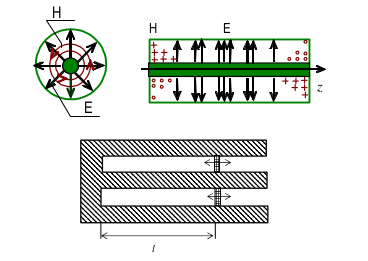
\includegraphics[scale=1]{14}$\\
\end{center}
\end{itemize}
\end{solution}